\section{Durchführung 501}

\subsection{Überprüfung der Proportionalität}

\begin{figure}[h!]
	\centering
	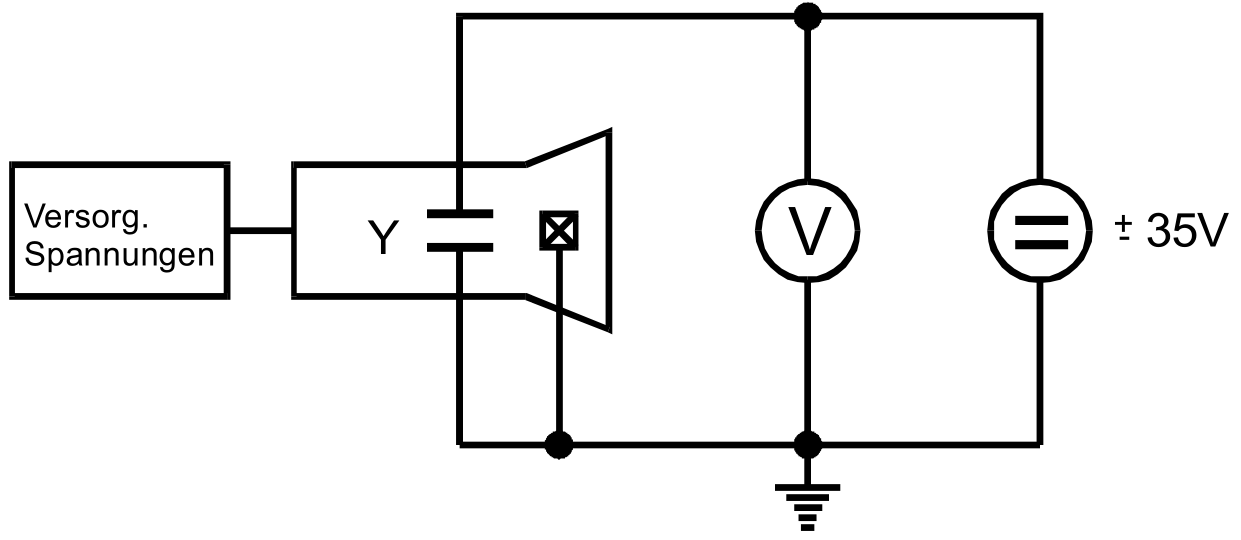
\includegraphics[width=1\linewidth]{aufbau1.png}
	\caption{Schaltbild des Kathodenstrahlrohrs}
	\label{fig:aufbau1}
\end{figure}
Zunächst wird mithilfe von Abbildung \ref{fig:aufbau1} die Kathodenstrahlröhre verschaltet. Zur Überprüfung der Proportionalität zwischen der Verschiebung $D$ des Leuchtflecks auf dem Schirm und der Ablenkspannung $U_{\text{d}}$ 
werden fünf verschiedene Beschleunigungsspannungen $U_{\text{B}}$ zwischen 180 und 500\,V gewählt. Für jedes $U_{\text{B}}$ wird dann $U_{\text{d}}$ so eingestellt, dass der Leuchtfleck auf einer der äquidistanten Linien 
des Schirms liegt, woraufhin die eingestellte Ablenkspannung $U_{\text{d}}$ abgelesen wird. Genauso wird dann für die weiteren acht Linien des Schirms vorgegangen. 



\subsection{Erzeugung stehender Wellen mittels Kathodenstrahl-Oszillographen}

\begin{figure}[h!]
	\centering
	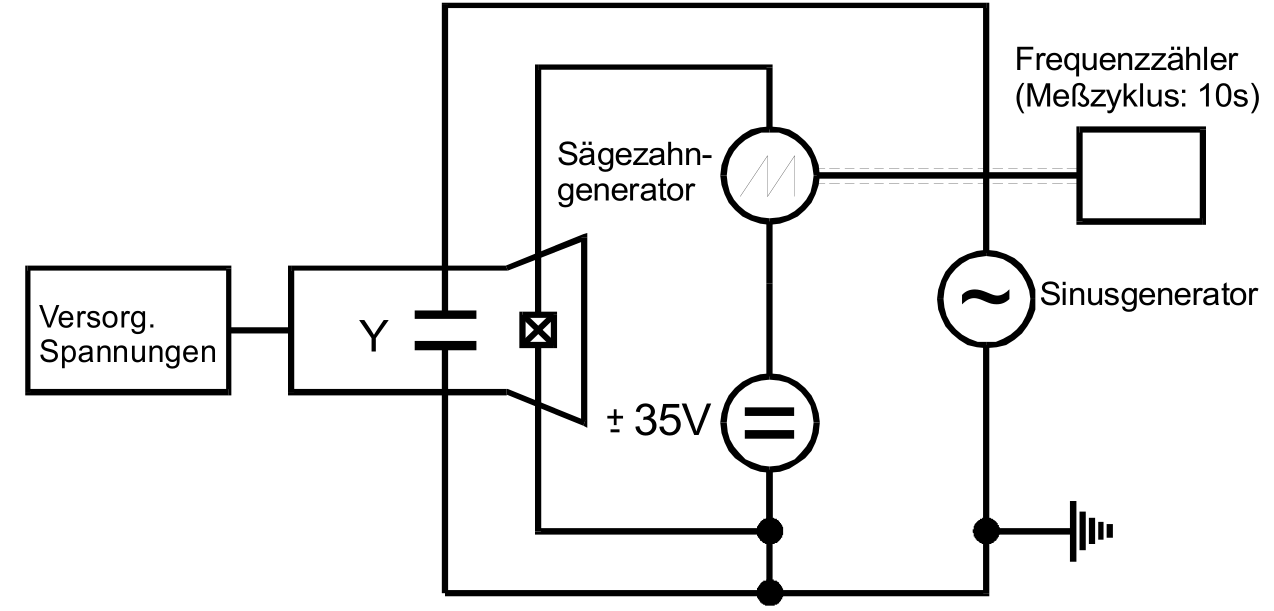
\includegraphics[width=1\linewidth]{aufbau2.png}
	\caption{Schaltbild des Kathodenstrahl-Oszillographen}
	\label{fig:aufbau2}
\end{figure}
Der Aufbau des Oszillographen erfolgt mithilfe der Abbildung \ref{fig:aufbau2}. Nun wird die Sägezahnfrequenz $\nu_{\text{Sä}}$ so eingestellt, dass sich ein stehendes Bild der Sinusspannung, welche vom Gerät vorgegeben eine 
Frequenz zwischen 80 und 90\,Hz hat, auf dem Schirm ergibt. Hierbei soll

\begin{equation*}
n \cdot \nu_{\text{Sä}} = \nu_{\text{Si}}
\end{equation*}
mit $n = \frac{1}{2}, 1, 2$ und 3 gelten. Für jedes $n$ wird die Sägezahnfrequenz notiert. Zuletzt wird die maximale Strahlauslenkung in Y-Richtung bei konstanter Beschleunigungsspannung abgemessen.